% Options for packages loaded elsewhere
\PassOptionsToPackage{unicode}{hyperref}
\PassOptionsToPackage{hyphens}{url}
%
\documentclass[
]{book}
\usepackage{amsmath,amssymb}
\usepackage{lmodern}
\usepackage{iftex}
\ifPDFTeX
  \usepackage[T1]{fontenc}
  \usepackage[utf8]{inputenc}
  \usepackage{textcomp} % provide euro and other symbols
\else % if luatex or xetex
  \usepackage{unicode-math}
  \defaultfontfeatures{Scale=MatchLowercase}
  \defaultfontfeatures[\rmfamily]{Ligatures=TeX,Scale=1}
\fi
% Use upquote if available, for straight quotes in verbatim environments
\IfFileExists{upquote.sty}{\usepackage{upquote}}{}
\IfFileExists{microtype.sty}{% use microtype if available
  \usepackage[]{microtype}
  \UseMicrotypeSet[protrusion]{basicmath} % disable protrusion for tt fonts
}{}
\makeatletter
\@ifundefined{KOMAClassName}{% if non-KOMA class
  \IfFileExists{parskip.sty}{%
    \usepackage{parskip}
  }{% else
    \setlength{\parindent}{0pt}
    \setlength{\parskip}{6pt plus 2pt minus 1pt}}
}{% if KOMA class
  \KOMAoptions{parskip=half}}
\makeatother
\usepackage{xcolor}
\IfFileExists{xurl.sty}{\usepackage{xurl}}{} % add URL line breaks if available
\IfFileExists{bookmark.sty}{\usepackage{bookmark}}{\usepackage{hyperref}}
\hypersetup{
  pdfauthor={Lecturer: Aslisho Qurboniev},
  hidelinks,
  pdfcreator={LaTeX via pandoc}}
\urlstyle{same} % disable monospaced font for URLs
\usepackage{color}
\usepackage{fancyvrb}
\newcommand{\VerbBar}{|}
\newcommand{\VERB}{\Verb[commandchars=\\\{\}]}
\DefineVerbatimEnvironment{Highlighting}{Verbatim}{commandchars=\\\{\}}
% Add ',fontsize=\small' for more characters per line
\usepackage{framed}
\definecolor{shadecolor}{RGB}{248,248,248}
\newenvironment{Shaded}{\begin{snugshade}}{\end{snugshade}}
\newcommand{\AlertTok}[1]{\textcolor[rgb]{0.94,0.16,0.16}{#1}}
\newcommand{\AnnotationTok}[1]{\textcolor[rgb]{0.56,0.35,0.01}{\textbf{\textit{#1}}}}
\newcommand{\AttributeTok}[1]{\textcolor[rgb]{0.77,0.63,0.00}{#1}}
\newcommand{\BaseNTok}[1]{\textcolor[rgb]{0.00,0.00,0.81}{#1}}
\newcommand{\BuiltInTok}[1]{#1}
\newcommand{\CharTok}[1]{\textcolor[rgb]{0.31,0.60,0.02}{#1}}
\newcommand{\CommentTok}[1]{\textcolor[rgb]{0.56,0.35,0.01}{\textit{#1}}}
\newcommand{\CommentVarTok}[1]{\textcolor[rgb]{0.56,0.35,0.01}{\textbf{\textit{#1}}}}
\newcommand{\ConstantTok}[1]{\textcolor[rgb]{0.00,0.00,0.00}{#1}}
\newcommand{\ControlFlowTok}[1]{\textcolor[rgb]{0.13,0.29,0.53}{\textbf{#1}}}
\newcommand{\DataTypeTok}[1]{\textcolor[rgb]{0.13,0.29,0.53}{#1}}
\newcommand{\DecValTok}[1]{\textcolor[rgb]{0.00,0.00,0.81}{#1}}
\newcommand{\DocumentationTok}[1]{\textcolor[rgb]{0.56,0.35,0.01}{\textbf{\textit{#1}}}}
\newcommand{\ErrorTok}[1]{\textcolor[rgb]{0.64,0.00,0.00}{\textbf{#1}}}
\newcommand{\ExtensionTok}[1]{#1}
\newcommand{\FloatTok}[1]{\textcolor[rgb]{0.00,0.00,0.81}{#1}}
\newcommand{\FunctionTok}[1]{\textcolor[rgb]{0.00,0.00,0.00}{#1}}
\newcommand{\ImportTok}[1]{#1}
\newcommand{\InformationTok}[1]{\textcolor[rgb]{0.56,0.35,0.01}{\textbf{\textit{#1}}}}
\newcommand{\KeywordTok}[1]{\textcolor[rgb]{0.13,0.29,0.53}{\textbf{#1}}}
\newcommand{\NormalTok}[1]{#1}
\newcommand{\OperatorTok}[1]{\textcolor[rgb]{0.81,0.36,0.00}{\textbf{#1}}}
\newcommand{\OtherTok}[1]{\textcolor[rgb]{0.56,0.35,0.01}{#1}}
\newcommand{\PreprocessorTok}[1]{\textcolor[rgb]{0.56,0.35,0.01}{\textit{#1}}}
\newcommand{\RegionMarkerTok}[1]{#1}
\newcommand{\SpecialCharTok}[1]{\textcolor[rgb]{0.00,0.00,0.00}{#1}}
\newcommand{\SpecialStringTok}[1]{\textcolor[rgb]{0.31,0.60,0.02}{#1}}
\newcommand{\StringTok}[1]{\textcolor[rgb]{0.31,0.60,0.02}{#1}}
\newcommand{\VariableTok}[1]{\textcolor[rgb]{0.00,0.00,0.00}{#1}}
\newcommand{\VerbatimStringTok}[1]{\textcolor[rgb]{0.31,0.60,0.02}{#1}}
\newcommand{\WarningTok}[1]{\textcolor[rgb]{0.56,0.35,0.01}{\textbf{\textit{#1}}}}
\usepackage{longtable,booktabs,array}
\usepackage{calc} % for calculating minipage widths
% Correct order of tables after \paragraph or \subparagraph
\usepackage{etoolbox}
\makeatletter
\patchcmd\longtable{\par}{\if@noskipsec\mbox{}\fi\par}{}{}
\makeatother
% Allow footnotes in longtable head/foot
\IfFileExists{footnotehyper.sty}{\usepackage{footnotehyper}}{\usepackage{footnote}}
\makesavenoteenv{longtable}
\usepackage{graphicx}
\makeatletter
\def\maxwidth{\ifdim\Gin@nat@width>\linewidth\linewidth\else\Gin@nat@width\fi}
\def\maxheight{\ifdim\Gin@nat@height>\textheight\textheight\else\Gin@nat@height\fi}
\makeatother
% Scale images if necessary, so that they will not overflow the page
% margins by default, and it is still possible to overwrite the defaults
% using explicit options in \includegraphics[width, height, ...]{}
\setkeys{Gin}{width=\maxwidth,height=\maxheight,keepaspectratio}
% Set default figure placement to htbp
\makeatletter
\def\fps@figure{htbp}
\makeatother
\setlength{\emergencystretch}{3em} % prevent overfull lines
\providecommand{\tightlist}{%
  \setlength{\itemsep}{0pt}\setlength{\parskip}{0pt}}
\setcounter{secnumdepth}{5}
\usepackage{booktabs}
\ifLuaTeX
  \usepackage{selnolig}  % disable illegal ligatures
\fi
\usepackage[]{natbib}
\bibliographystyle{plainnat}

\title{The Medieval Islamicate World: 570-1250

تاريخ الإسلام}
\author{Lecturer: Aslisho Qurboniev}
\date{2022-05-02}

\usepackage{amsthm}
\newtheorem{theorem}{Theorem}[chapter]
\newtheorem{lemma}{Lemma}[chapter]
\newtheorem{corollary}{Corollary}[chapter]
\newtheorem{proposition}{Proposition}[chapter]
\newtheorem{conjecture}{Conjecture}[chapter]
\theoremstyle{definition}
\newtheorem{definition}{Definition}[chapter]
\theoremstyle{definition}
\newtheorem{example}{Example}[chapter]
\theoremstyle{definition}
\newtheorem{exercise}{Exercise}[chapter]
\theoremstyle{definition}
\newtheorem{hypothesis}{Hypothesis}[chapter]
\theoremstyle{remark}
\newtheorem*{remark}{Remark}
\newtheorem*{solution}{Solution}
\begin{document}
\maketitle

{
\setcounter{tocdepth}{1}
\tableofcontents
}
\hypertarget{course-description}{%
\chapter{Course description}\label{course-description}}

The aim of this course is to provide an introduction to the early history of the Islamic world, from the rise of Islam in Arabia to the formation of a world civilisation. Students will learn how to relate ideas to historical, geographical, and material factors. Particular attention will be paid to religious and cultural continuity, as a backdrop to the evolution of an Islamic identity and institutions of government, administration, and education.

\hypertarget{intended-learning-outcomes}{%
\section{Intended learning outcomes}\label{intended-learning-outcomes}}

\begin{enumerate}
\def\labelenumi{\arabic{enumi}.}
\tightlist
\item
  Students will learn about the most important developments in Islamic history, main questions in the historiography of Islam, and be able to reflect historically and critically.
\item
  They should be able to find their way around major reference works for Islamic history and gain some familiarity with some primary sources.
\item
  They will learn how to write critical essays following the conventions of style and referencing in the field of Islamic history.
\item
  They will be able to apply the skills and methodological approaches to other subjects of study. They should be able to situate topics from Islamic studies in their historical context.
\end{enumerate}

\hypertarget{lectures}{%
\section{Lectures}\label{lectures}}

Weekly lectures will cover the period from the rise of Islam in Late Antiquity to the decline of the major caliphates and the appearances of new polities ruled mostly by non-Arabs. This historical shift is marked by the takeover of Baghdad by the Seljuq Turks on the one hand, and the breakup of Ifrīqiya (Tunisia) under the Berber Zirids from the Fatimid empire in 1050s on the other. Each lecture will highlight historiographical issues, which will then be picked up during the seminars.

\hypertarget{seminars}{%
\section{Seminars}\label{seminars}}

Seminars will follow the themes of the lectures but will expect input from students. For this, in addition to the discussion of secondary sources, students will be expected to engage with short excerpts from primary sources listed in the syllabus. Presentations will also take place during the seminars.

To prepare for the seminars you must read the weekly readings listed first closely as these will provide you with the general framework. Reading these will help you to be more selective about books and articles recommended for further reading. The short primary source readings are also essential for the seminars. All of this will help you with the exams.

\begin{verbatim}
\end{verbatim}

\hypertarget{assessment}{%
\section{Assessment}\label{assessment}}

Essay (50\%), open-book exam (30\%), presentation (15\%), participation (5\%).

\emph{Essay,} of maximum 2500 words. Essay questions will be drawn from the lectures and seminars topics and will be given one week before the submission date. You will be expected to be able to connect several topics and draw upon readings from several weeks, in addition to topic specific readings which will be provided with the questions.

\emph{Open-book exam.} The questions for open-book exam will be based on the list of books provided in the end of this syllabus. You will be asked to answer one of the questions within three hours, drawing on your knowledge of the course materials. The response must demonstrate a good overall understanding of the topics of Islamic history, an ability to select relevant material, and a close engagement with the selected books that you will have access to during the exam. You will not be penalised for poor referencing, spelling mistakes, and typos.

\emph{Presentation.} You will choose to present on one of the weekly topics, during one of the seminars. A strong presentation will combine a good understanding of the readings and an engaging and convincing use of material and archaeological evidence.

\emph{Participation.} It is essential to attend the lectures and seminars. You will be marked on your contributions to class discussions.

\hypertarget{resources-and-reading-materials}{%
\section{Resources and reading materials}\label{resources-and-reading-materials}}

\hypertarget{reference-works}{%
\subsection{Reference Works}\label{reference-works}}

\begin{itemize}
\tightlist
\item
  Bosworth, C. E. The Islamic Dynasties: A Chronological and Geneological Manual. Ediburgh, 2004.
\item
  Encyclopaedia of Islam, 2nd and 3rd Editions (online)
\item
  Encycloaedia Islamica (online)
\item
  Encyclopaedia Iranica (online)
\item
  Index Islamicus (online)
\item
  Oxford Islamic Studies Online
\item
  The Cambridge History of the Byzantine Empire (online)
\item
  The Cambridge History of Egypt (online)
\item
  The New Cambridge History of Islam (online)
\item
  The Cambridge History of Iran (online)
\end{itemize}

\hypertarget{textbooks}{%
\subsection{Textbooks}\label{textbooks}}

\begin{itemize}
\tightlist
\item
  Berkey, Jonathan. The Formation of Islam: Religion and Society in the Near East, 600-1800. Cambridge, 2002.
\item
  Hodgson, Marshall. The Venture of Islam: Conscience and History in a World Civilisation. Vol. 1: The Classical Age of Islam and Volume 2: The Expansion of Islam in the Middle Periods. Chicago and London, 1977.
\end{itemize}

\hypertarget{surveys}{%
\subsection{Surveys}\label{surveys}}

\begin{itemize}
\tightlist
\item
  Barthold, Vasiliĭ V. Turkestan down to the Mongol Invasion, 3rd ed.~London, 1968.
\item
  Brett, Michael and Elizabeth Fentress. The Berbers. Oxford, 1996.
\item
  Bulliet, Richard. Islam: The View from the Edge. New York, 1994.
\item
  Hitchcock, Richard. Muslim Spain Reconsidered: From 711 to 1502. Edinburgh, 2014, 1-121.
\item
  Lapidus, Ira. A History of Islamic Societies, 2nd ed.~Cambridge, 2002.
\item
  Kennedy, Hugh. Muslim Spain and Portugal: a political history of al-Andalus. London and New York, 1996.
\item
  Kennedy, Hugh. The Prophet and the Age of the Caliphate. Harlow, UK, 2004.
\item
  Silverstein, Adam. Islamic History: A Very Short Introduction. Oxford, 2010.
\item
  van Steenbergen, Jo. A History of the Islamic World, 600-1800. London and New York, 2021.
\end{itemize}

\hypertarget{historiography}{%
\subsection{Historiography}\label{historiography}}

\begin{itemize}
\tightlist
\item
  Anthony, Sean. Muhammad and the Empires of Faith: The Making of the Prophet of Islam. Oakland, 2020.
\item
  Donner, Fred. Narratives of Islamic Origins: The beginning of Islamic Historical Writing. Princeton, 1998.
\item
  Humphreys, Stephen. Islamic History: A Framework for Inquiry, Revised Edition. London, 2009.
\item
  Hoyland, Robert. Seeing Islam as others saw it: a survey and evaluation of Christian, Jewish, and Zoroastrian writings on early Islam. Princeton, 1997.
\item
  Khalidi, Tarif. Arabic Historical thought in the Classical Period. Cambridge, 1994.
\item
  Melville, Charles and Jürgen Paul (eds.) Persian L0cal Histories, Special issue of Iranian Studies 33 (1-2).
\item
  Robinson, Chase. Islamic Historiography. Cambridge, 2003.
\item
  Rozenthal, Franz. A History of Muslim Historiography, 2nd ed.~Leiden, 1968.
\end{itemize}

\hypertarget{week-1.-introduction}{%
\chapter{Week 1. Introduction}\label{week-1.-introduction}}

All chapters start with a first-level heading followed by your chapter title, like the line above. There should be only one first-level heading (\texttt{\#}) per .Rmd file.

\hypertarget{a-section}{%
\section{A section}\label{a-section}}

All chapter sections start with a second-level (\texttt{\#\#}) or higher heading followed by your section title, like the sections above and below here. You can have as many as you want within a chapter.

\hypertarget{an-unnumbered-section}{%
\subsection*{An unnumbered section}\label{an-unnumbered-section}}
\addcontentsline{toc}{subsection}{An unnumbered section}

Chapters and sections are numbered by default. To un-number a heading, add a \texttt{\{.unnumbered\}} or the shorter \texttt{\{-\}} at the end of the heading, like in this section.

\hypertarget{week-2-the-rise-of-islam-in-late-antiquity}{%
\chapter{Week 2: The Rise of Islam in Late Antiquity}\label{week-2-the-rise-of-islam-in-late-antiquity}}

Cross-references make it easier for your readers to find and link to elements in your book.

\hypertarget{chapters-and-sub-chapters}{%
\section{Chapters and sub-chapters}\label{chapters-and-sub-chapters}}

There are two steps to cross-reference any heading:

\begin{enumerate}
\def\labelenumi{\arabic{enumi}.}
\tightlist
\item
  Label the heading: \texttt{\#\ Hello\ world\ \{\#nice-label\}}.

  \begin{itemize}
  \tightlist
  \item
    Leave the label off if you like the automated heading generated based on your heading title: for example, \texttt{\#\ Hello\ world} = \texttt{\#\ Hello\ world\ \{\#hello-world\}}.
  \item
    To label an un-numbered heading, use: \texttt{\#\ Hello\ world\ \{-\#nice-label\}} or \texttt{\{\#\ Hello\ world\ .unnumbered\}}.
  \end{itemize}
\item
  Next, reference the labeled heading anywhere in the text using \texttt{\textbackslash{}@ref(nice-label)}; for example, please see Chapter \ref{cross}.

  \begin{itemize}
  \tightlist
  \item
    If you prefer text as the link instead of a numbered reference use: \protect\hyperlink{cross}{any text you want can go here}.
  \end{itemize}
\end{enumerate}

\hypertarget{captioned-figures-and-tables}{%
\section{Captioned figures and tables}\label{captioned-figures-and-tables}}

Figures and tables \emph{with captions} can also be cross-referenced from elsewhere in your book using \texttt{\textbackslash{}@ref(fig:chunk-label)} and \texttt{\textbackslash{}@ref(tab:chunk-label)}, respectively.

See Figure \ref{fig:nice-fig}.

\begin{Shaded}
\begin{Highlighting}[]
\FunctionTok{par}\NormalTok{(}\AttributeTok{mar =} \FunctionTok{c}\NormalTok{(}\DecValTok{4}\NormalTok{, }\DecValTok{4}\NormalTok{, .}\DecValTok{1}\NormalTok{, .}\DecValTok{1}\NormalTok{))}
\FunctionTok{plot}\NormalTok{(pressure, }\AttributeTok{type =} \StringTok{\textquotesingle{}b\textquotesingle{}}\NormalTok{, }\AttributeTok{pch =} \DecValTok{19}\NormalTok{)}
\end{Highlighting}
\end{Shaded}

\begin{figure}

{\centering 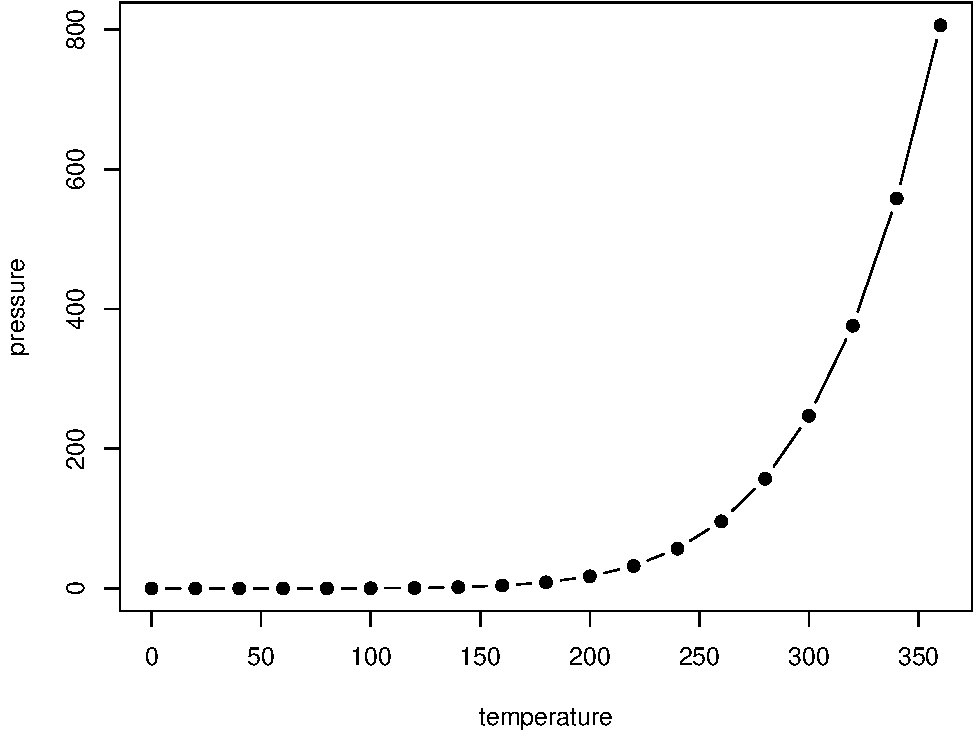
\includegraphics[width=0.8\linewidth]{_main_files/figure-latex/nice-fig-1} 

}

\caption{Here is a nice figure!}\label{fig:nice-fig}
\end{figure}

Don't miss Table \ref{tab:nice-tab}.

\begin{Shaded}
\begin{Highlighting}[]
\NormalTok{knitr}\SpecialCharTok{::}\FunctionTok{kable}\NormalTok{(}
  \FunctionTok{head}\NormalTok{(pressure, }\DecValTok{10}\NormalTok{), }\AttributeTok{caption =} \StringTok{\textquotesingle{}Here is a nice table!\textquotesingle{}}\NormalTok{,}
  \AttributeTok{booktabs =} \ConstantTok{TRUE}
\NormalTok{)}
\end{Highlighting}
\end{Shaded}

\begin{table}

\caption{\label{tab:nice-tab}Here is a nice table!}
\centering
\begin{tabular}[t]{rr}
\toprule
temperature & pressure\\
\midrule
0 & 0.0002\\
20 & 0.0012\\
40 & 0.0060\\
60 & 0.0300\\
80 & 0.0900\\
\addlinespace
100 & 0.2700\\
120 & 0.7500\\
140 & 1.8500\\
160 & 4.2000\\
180 & 8.8000\\
\bottomrule
\end{tabular}
\end{table}

\hypertarget{week-3.-muhammad-and-his-successors}{%
\chapter{Week 3. Muhammad and his successors}\label{week-3.-muhammad-and-his-successors}}

You can add parts to organize one or more book chapters together. Parts can be inserted at the top of an .Rmd file, before the first-level chapter heading in that same file.

Add a numbered part: \texttt{\#\ (PART)\ Act\ one\ \{-\}} (followed by \texttt{\#\ A\ chapter})

Add an unnumbered part: \texttt{\#\ (PART\textbackslash{}*)\ Act\ one\ \{-\}} (followed by \texttt{\#\ A\ chapter})

Add an appendix as a special kind of un-numbered part: \texttt{\#\ (APPENDIX)\ Other\ stuff\ \{-\}} (followed by \texttt{\#\ A\ chapter}). Chapters in an appendix are prepended with letters instead of numbers.

\hypertarget{week-4.-the-umayyads-an-arab-islamic-monarchy}{%
\chapter{Week 4. The Umayyads: an Arab-Islamic monarchy}\label{week-4.-the-umayyads-an-arab-islamic-monarchy}}

\hypertarget{footnotes}{%
\section{Footnotes}\label{footnotes}}

Footnotes are put inside the square brackets after a caret \texttt{\^{}{[}{]}}. Like this one \footnote{This is a footnote.}.

\hypertarget{citations}{%
\section{Citations}\label{citations}}

Reference items in your bibliography file(s) using \texttt{@key}.

For example, we are using the \textbf{bookdown} package \citep{R-bookdown} (check out the last code chunk in index.Rmd to see how this citation key was added) in this sample book, which was built on top of R Markdown and \textbf{knitr} \citep{xie2015} (this citation was added manually in an external file book.bib).
Note that the \texttt{.bib} files need to be listed in the index.Rmd with the YAML \texttt{bibliography} key.

The RStudio Visual Markdown Editor can also make it easier to insert citations: \url{https://rstudio.github.io/visual-markdown-editing/\#/citations}

\hypertarget{week-5.-the-ux2bfabbasids-an-islamic-empire}{%
\chapter{Week 5. The ʿAbbasids: an Islamic empire}\label{week-5.-the-ux2bfabbasids-an-islamic-empire}}

\hypertarget{equations}{%
\section{Equations}\label{equations}}

Here is an equation.

\begin{equation} 
  f\left(k\right) = \binom{n}{k} p^k\left(1-p\right)^{n-k}
  \label{eq:binom}
\end{equation}

You may refer to using \texttt{\textbackslash{}@ref(eq:binom)}, like see Equation \eqref{eq:binom}.

\hypertarget{theorems-and-proofs}{%
\section{Theorems and proofs}\label{theorems-and-proofs}}

Labeled theorems can be referenced in text using \texttt{\textbackslash{}@ref(thm:tri)}, for example, check out this smart theorem \ref{thm:tri}.

\begin{theorem}
\protect\hypertarget{thm:tri}{}\label{thm:tri}For a right triangle, if \(c\) denotes the \emph{length} of the hypotenuse
and \(a\) and \(b\) denote the lengths of the \textbf{other} two sides, we have
\[a^2 + b^2 = c^2\]
\end{theorem}

Read more here \url{https://bookdown.org/yihui/bookdown/markdown-extensions-by-bookdown.html}.

\hypertarget{callout-blocks}{%
\section{Callout blocks}\label{callout-blocks}}

The R Markdown Cookbook provides more help on how to use custom blocks to design your own callouts: \url{https://bookdown.org/yihui/rmarkdown-cookbook/custom-blocks.html}

\hypertarget{week-6.-conversion-to-islam-and-the-non-muslim-communities}{%
\chapter{Week 6. Conversion to Islam and the non-Muslim communities}\label{week-6.-conversion-to-islam-and-the-non-muslim-communities}}

\hypertarget{publishing}{%
\section{Publishing}\label{publishing}}

HTML books can be published online, see: \url{https://bookdown.org/yihui/bookdown/publishing.html}

\hypertarget{pages}{%
\section{404 pages}\label{pages}}

By default, users will be directed to a 404 page if they try to access a webpage that cannot be found. If you'd like to customize your 404 page instead of using the default, you may add either a \texttt{\_404.Rmd} or \texttt{\_404.md} file to your project root and use code and/or Markdown syntax.

\hypertarget{metadata-for-sharing}{%
\section{Metadata for sharing}\label{metadata-for-sharing}}

Bookdown HTML books will provide HTML metadata for social sharing on platforms like Twitter, Facebook, and LinkedIn, using information you provide in the \texttt{index.Rmd} YAML. To setup, set the \texttt{url} for your book and the path to your \texttt{cover-image} file. Your book's \texttt{title} and \texttt{description} are also used.

This \texttt{gitbook} uses the same social sharing data across all chapters in your book- all links shared will look the same.

Specify your book's source repository on GitHub using the \texttt{edit} key under the configuration options in the \texttt{\_output.yml} file, which allows users to suggest an edit by linking to a chapter's source file.

Read more about the features of this output format here:

\url{https://pkgs.rstudio.com/bookdown/reference/gitbook.html}

Or use:

\begin{Shaded}
\begin{Highlighting}[]
\NormalTok{?bookdown}\SpecialCharTok{::}\NormalTok{gitbook}
\end{Highlighting}
\end{Shaded}


  \bibliography{book.bib,packages.bib}

\end{document}
